\hypertarget{6}{}

\rhead{A Hybrid Approach toward Biomedical Relation Extraction Training Corpora}
\lhead{Chapter 6}

\chapter[A Hybrid Approach toward Biomedical Relation Extraction Training Corpora: Combining Distant Supervision with Crowdsourcing]
{\huge A Hybrid Approach toward Biomedical Relation Extraction Training Corpora: Combining Distant Supervision with Crowdsourcing \\
\Large \textmd{Diana Sousa, Andre Lamurias, and Francisco M. Couto}}

\vspace{-1.6cm}

% Gray Line
\begingroup
\color{black}
\par\noindent\rule{\textwidth}{0.4pt}
\endgroup

\noindent{This chapter tackles Objective 2 by demonstrating the possibility of creating \acl{RE} (RE) training data using distant supervision allied with crowdsourcing and corresponds to the journal article:} 

\begin{itemize}[label=]
    \item{\textbf{Sousa, D.}, Lamurias, A., and Couto, F. M. (2020). \textbf{A Hybrid Approach Toward Biomedical Relation Extraction Training Corpora: Combining Distant Supervision with Crowdsourcing}. Database, 2020:1-15. (Q1 Scimago) \citep{sousa2020hybrid}} 
\end{itemize}

\noindent{\textbf{Abstract.} Biomedical RE datasets are vital in the construction of knowledge bases and potentiate the discovery of new interactions. There are several ways to create biomedical RE datasets, some more reliable than others, such as using domain expert annotations. However, the emerging use of crowdsourcing platforms, such as Amazon Mechanical Turk (MTurk), can potentially reduce the cost of RE dataset construction, even if the same level of quality cannot be guaranteed. There is a lack of power for the researcher to control who, how and in what context workers engage in crowdsourcing platforms. Hence, allying distant supervision with crowdsourcing can be a more reliable alternative. The crowdsourcing workers would be asked only to rectify or discard already existing annotations, making the process less dependent on their ability to interpret complex biomedical sentences. In this work, we use a previously created distantly supervised human phenotype–gene relations (PGR) dataset to perform crowdsourcing validation. We divided the original dataset into two annotation tasks: Task 1, 70\% of the dataset annotated by one worker, and Task 2, 30\% of the dataset annotated by seven workers. Also, for Task 2, we added an extra rater on-site and a domain expert to further assess the crowdsourcing validation quality. Here, we describe a detailed pipeline for RE crowdsourcing validation, create a new release of the PGR dataset with partial domain expert revision, and assess the quality of the MTurk platform. We applied the new dataset to two state-of-the-art deep learning systems (BiOnt and BioBERT) and compared its performance with the original PGR dataset, as well as combinations between the two, achieving a 0.3494 increase in average F-measure. The code supporting our work and the new release of the PGR dataset is available at \url{https://github.com/lasigeBioTM/PGR-crowd.}}


\section{Introduction}

Knowledge bases play a fundamental role in the way we store, organize and retrieve information. More specifically, biological knowledge bases are commonplace for researchers and clinicians to access all types of biomedical data retrieved from biomedical literature \citep{arnaboldi2020text}. Previous works annotated biomedical literature by resorting to domain expert annotators \citep{herrero2013ddi}, crowdsourcing platforms \citep{tsueng2020applying}, or distantly supervised techniques \citep{sousa2019silver}. The main aim of these researchers is to tackle the lack of annotated datasets for biomedical information extraction systems. However, when applying distantly supervised techniques, the annotations are not as reliable as when done by domain experts, and it still needs to be adequately reviewed before the extracted information can be added to any biomedical repository. Hence, the added advantage of automating the extraction of information using distant supervision is slightly impaired by the need to review it, which is not only costly but time and resource-consuming.  Moreover, when targeting Relation Extraction (RE) between entities of different domains or document summarization tasks \citep{narayan2018ranking}, the revision process becomes cumbersome when compared to other information extraction tasks, given its higher complexity that normally requires knowledge of multiple domains. 

The alternative way to create reliable gold standard datasets that do not resort to domain expert curation could be allying distant supervision with crowdsourcing \citep{gormley2010non,liu2016effective,collovini2018annotating}. Before integrating data extracted from distant supervision pipelines into biological knowledge bases or using it as training data for biomedical information extraction systems, the data would go through a confirmation or review phase in the form of crowdsourcing. Crowdsourcing platforms are becoming increasingly popular to address the problem of lack of training corpora for natural language processing (NLP) tasks \citep{callison2010creating}. Currently, the most popular platform for this purpose is Amazon Mechanical Turk (MTurk) \citep{ipeirotis2010quality,yetisgen2010preliminary,khare2015scaling}. Some platforms created a trust layer over MTurk to facilitate task specification and monitoring \citep{wang2013perspectives}, such as Figure Eight (previously known as CrowdFlower) \citep{li2016crowdsourcing,feyisetan2015towards}, which is widely used by researchers for biomedical NLP related tasks. 

One of the problems of using crowdsourcing platforms is the lack of domain expertise. While most platforms allow us to specify some criteria (e.g., degree of education) in exchange for an increased price per task, it is not feasible to specify expertise in particular biomedical domains. Not only that, but there is no guarantee that the quality promised is the quality provided because some malicious workers often take advantage of the difficulty in implementing a verification procedure and submit answers of low quality \citep{callison2010creating}. Task redundancy can be a solution, but it also increases the costs of using crowdsourcing approaches, partially defeating the purpose of these platforms. The question should be whether the quality of the workers is good enough for the purpose of the task and if the difference in quality when compared to domain experts is compensated by the decrease in costs. In the case of the MTurk platform, some studies have supported its suitability for various tasks \citep{mortensen2018comparing}. However, it fails in transparency about its workers' context (e.g., background), if MTurk constitutes their primary form of income or not, what is their motivation for completing the tasks, and if this introduces bias to the tasks at hand. These and other ethical questions have been discussed in depth by some researchers \citep{fort2011amazon,paolacci2014inside}.

In this work, we leveraged an existing dataset of biomedical relations created through distant supervision and submitted it to the MTurk platform for crowdsourcing validation. With the exhaustive review of the performance of the original and new datasets, we assessed the viability of combining distant supervision and crowdsourcing for the field of biomedical RE. 

Our work used an open-source dataset, the PGR dataset \citep{sousa2019silver}, based on distant supervision, that features both human phenotype and gene annotations and their relations. Since it is a silver standard dataset, it has not been reviewed by domain experts, leading to wrongly labelled relations and other errors. These errors can be from Named-Entity Recognition (NER) (e.g., acronyms of diseases annotated as genes), which was also done automatically, or sentence format errors. To rectify these errors, we used the MTurk platform to validate, alter, or discard the relations within the PGR dataset. We achieved this by dividing the original dataset into two partitions, one of 70\% (Task 1), where each relation was rated by one Amazon worker, and another of 30\% (Task 2), where each relation was rated by seven distinct workers. We validated our approach through inter-rater agreement using the Fleiss’ kappa \citep{mchugh2012interrater} and the  Krippendorff’s alpha \citep{krippendorff2011computing} metrics for Task 2. Further, we also provided the 30\% partition of the PGR dataset used for Task 2 to an external rater (on-site, without previous curating experience but holding a Biochemistry degree) and to a domain expert (with previous curating experience, holding a PhD in Bioinformatics). These different levels of expertise enlightened the difficulties of curating the dataset and the limitations associated with each level. To evaluate and compare the quality of the crowdsourced Amazon dataset, we applied it to two state-of-the-art deep learning systems and compared its performance with the original PGR dataset, as well as combinations between the two. The deep learning systems used were BiOnt \citep{sousa2020biont} and BioBERT \citep{lee2020biobert}, that feature relation extraction between different biomedical entities with high performance, and, in the case of BiOnt, it was already used in conjunction with the PGR dataset. 

The performance of the MTurk workers in comparison with our on-site curator and the domain expert was generally good for accessing NER or sentence format errors (approximately 16\% of relations). However, the MTurk workers struggle to identify false relations (separate entities without association in a sentence). The struggle to identify these relations can be due to the complexity of the sentences or quality issues related to the MTurk platform validation of workers, which we will discuss in more detail in the following sections. Further, the inter-rater agreement for Task 2 showed a slight to a fair agreement (about 0.20-0.21), which is below what we expected and we believe could be related to the problems of sentence complexity and quality reported.  Regarding the performance of the crowdsourced Amazon dataset in the application of the BiOnt and BioBERT systems, we had an average increase of 0.3494 in F-measure, taking into account all the experiences concerning the original PGR dataset. 
 
The main takeaways of this work were the need for further validation of the use of crowdsourcing platforms, such as the MTurk platform, and the potential of using distant supervision allied with crowdsourcing to produce gold standard datasets with which we can train viable models and detect relevant biomedical relations. This work resulted in the following contributions:

\begin{itemize}
    \item Pipeline for RE crowdsourcing, in which we describe in detail all the base concepts and steps taken to produce the new crowdsourced dataset.
    \item New release of the PGR Dataset, which will be made freely available to the community.
    \item Assessment of the quality of results obtained with the MTurk platform (through statistical analysis and direct comparison with on-site rater and domain expert).
\end{itemize}

\section{Materials and Methods}

This section presents an overview of the PGR dataset \citep{sousa2019silver}, a brief presentation of the Amazon Mechanical Turk (MTurk) platform, and the integration of the dataset into the MTurk platform (including the design, configuration, and evaluation stages). We now describe how we proceeded with each of these stages: 

\begin{enumerate}
    \item Design
    \begin{enumerate}
        \item Set up the tasks (Human Intelligence Task - HIT) to be simple to understand and easy to accomplish by the employees (i.e., workers or turkers).
        \item Define the guidelines (instructions) with examples for the workers to better understand the presented HITs. 
    \end{enumerate}
    \item Configuration
    \begin{enumerate}
        \item Configure the MTurk platform specifying different criteria (for workers) and wages (i.e., reward).
        \item Submit the HITs within the platform.
    \end{enumerate}
    \item Evaluation
    \begin{enumerate}
        \item Calculate inter-rater agreement.
        \item Compare  the PGR dataset before and after MTurk crowdsourcing assessment by employing  two different deep learning models (BiOnt \citep{sousa2020biont} and BioBERT \citep{lee2020biobert}).
    \end{enumerate}
\end{enumerate}

An overview of the pipeline of the work described in this paper can be found in Figure \ref{fig61}.

\begin{figure}
\centering
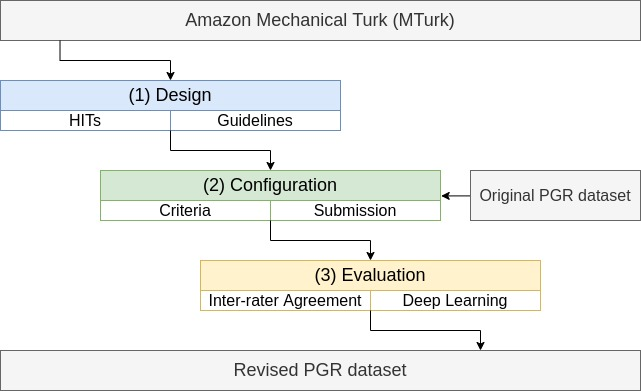
\includegraphics[width=0.8\linewidth]{images/chapter_6/figure_1.jpg}
\caption[Pipeline to Incorporate the PGR Dataset into MTurk]{The pipeline to incorporate the PGR dataset into the Amazon Mechanical Turk (MTurk) platform, including the design, configuration, and evaluation stages.} \label{fig61}
\end{figure}

\subsection{PGR Dataset}

The PGR dataset is a silver standard corpus of PubMed abstracts featuring human phenotype and gene annotations and their relations \citep{sousa2019silver}. In this dataset, all the annotations were generated in a fully automated fashion (silver standard), taking a distant supervision approach, opposite to a manually annotated dataset where domain experts generate the annotations (gold standard). 

The first release of the  PGR dataset focused mostly on the initial release of the dataset (10/12/2018), where a small subset of relations (6\%) was manually reviewed to evaluate the PGR dataset quality and also to use as a test corpus for machine learning model evaluation. The second release (11/03/2019) captured a more clear-cut search of the type of abstracts to retrieve, such as abstracts regarding diseases, their associated phenotypes and genes, increasing from about 2.5 relations per abstract to about 3.0 relations per abstract, and the overall number of relations by 2-fold. In this work, we are going to use the second release of the PGR dataset to generate an improved third release. 

The relations identified in the PGR dataset are either Known if present in the knowledge base of relations provided by the Human Phenotype Ontology (HPO) group \citep{kohler2017human} or Unknown otherwise. Table \ref{tab1} presents the numbers for the second release of the PGR dataset.

\begin{table}[h]
\centering
\caption[General Statistics for the PGR Dataset]{The number of abstracts, phenotype and gene annotations, and of known, unknown and total of relations for the second release (11/03/2019) of the PGR dataset (partial table from \citep{sousa2019silver})}\label{tab1}
\begin{tabular}{cccccc}
\hline
\multirow{2}{*}{Abstracts} & \multicolumn{2}{c}{Annotations} & \multicolumn{3}{c}{Relations} \\
\cline{2-6}
& Phenotype & Gene & Known & Unknown & Total \\
\hline
2657 & 9553 & 23786 & 2480 & 5483 & 7963 \\
\hline
\end{tabular}
\end{table}

\subsection{Amazon Mechanical Turk}

The Amazon Mechanical Turk (MTurk) is a crowdsourcing web service (marketplace) that facilitates the use of human intelligence by individuals and businesses that are in demand to complete specific tasks \citep{paolacci2010running}. In this web service, the employees (i.e., workers or turkers) execute tasks (i.e., HITs) submitted by employers (i.e., requesters) to earn a predefined wage (i.e., reward). The type of HITs that MTurk allows requesters to submit ranges from sentiment analysis and document classification in the language domain to image classification in the vision domain. Requesters post HITs to workers who meet their specified criteria (e.g., degree of education) and predefined both a reward and maximum time allotted for completing each task. Both requesters and workers remain anonymous throughout the process (workers can be identified through an internal identifier provided by Amazon). 

The three main benefits of the MTurk platform are: (1) optimized efficiency by allowing requesters to outsource tasks that need to be handled manually but do not require the requester or their employees' expertise; (2) increased flexibility for requesters to quickly scale their businesses without needing to scale their in-house workforce, and (3) cost reduction by eliminating the need for requesters to employ a temporary workforce and all the management costs associated with it \citep{ipeirotis2010quality}.

Some previous works using MTurk in the biomedical field include named-entity recognition and curation of biomedical entities labels’. \cite{yetisgen2010preliminary} used MTurk to extract named entities, such as medical conditions, medication, and laboratory tests, from clinical trial descriptions. \cite{good2014microtask} used it for disease mention annotation in PubMed abstracts. Similarly to our approach, \cite{khare2015scaling} used MTurk to curate indications from drug labels, i.e., to judge whether a drug is used in managing a highlighted disease.

\subsection{Integration into Amazon Mechanical Turk Platform}

The MTurk platform provides a wide range of customizable templates to start a new project. The template closest to our previously described curation task was the Document Classification template within the Language field that we leveraged to set up our PGR HITs. To facilitate the evaluation of the workers' performance, we divided the original dataset into partitions of 70\% (Task 1), where each relation was rated by one Amazon worker and 30\% (Task 2), where each relation was rated seven times by seven distinct workers. We also had to define guidelines (instructions) with examples for the workers to understand the task at hand thoroughly. Further, each project required defining criteria to select the workers that better suited the goals of the project and determining the reward per HIT for each worker before submission. Finally, after receiving the results (which took about two weeks), we had to evaluate the performance of our workers. The evaluation was done by calculating the inter-rater agreement and by comparing the performance of the PGR dataset before and after curation with existing deep learning tools.  

We describe the detailed steps that we took and the reasoning for each decision made in the following sections. 

\subsubsection{Design}

\paragraph{HITs}

As stated previously, we adapted the Document Classification template to set up our HITs. Thus, the workers were presented with a sentence with two entities in bold (the human phenotype and the gene entities) and a set of three possible classifications (true relation, false relation, or wrongly labelled relations due to errors in the NER stage or wrong sentence format). Figure \ref{fig2} represents an example of a HIT as presented to the workers (Task 2).

\begin{figure}
\centering
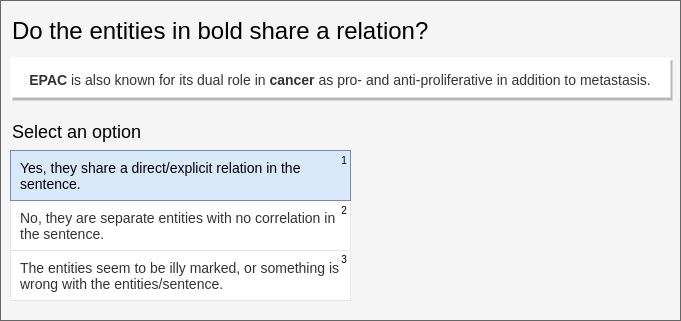
\includegraphics[width=0.8\linewidth]{images/chapter_6/figure_2.jpg}
\caption[HIT Example]{An example of a HIT presented to the workers and the available options.} \label{fig2}
\end{figure}

\paragraph{Guidelines}

In this work, we considered that rather than defining strict guidelines, it would be more intuitive for the workers to be presented with examples of instances and their gold labels (Supplementary Material Figure \ref{sfig1}). Nonetheless, the primary goal of the task presented to the workers was: The goal is to choose among three possible options to classify the relation between a phenotype and a gene in each sentence. The guidelines presented to the workers are illustrated by Supplementary Material Figure \ref{sfig1}. We opted out of more exhaustive guidelines to keep the task time manageable and more straightforward to understand.

\subsubsection{Configuration}

\paragraph{Criteria}

As we stated before, requesters can predefine specific criteria that the workers have to meet to be able to work on a task. However, specifying that criteria has an added cost per HIT that would make the total value for the task too expensive, invalidating the use of the crowd (domain expertise would be about the same value). Therefore, the criteria chosen and the cost of the crowdsourcing project described in this work are detailed in Table \ref{tab2}. The requirement that workers be ``Masters" (high-performing workers according to MTurk) adds \$0.001 to the Mechanical Turk Fee, but since the platform rounds it up to the cent, the total value is unaltered.

\begin{table}[h]
\centering
\caption[Summary of the Crowdsourcing Tasks Criteria and Associated Costs]{Summary of the crowdsourcing tasks criteria and associated costs}\label{tab2}
\begin{tabular}{lcc}
\hline
Setting & Task 1 & Task 2 \\
\hline
Reward per assignment (USD) & 0.02 & 0.02 \\
Mechanical Turk fee (USD) & 0.01 & 0.01 \\
Number of assignments per task & 1 & 7 \\
Minimum time per assignment & 3s & 3s \\
Require that Workers be Masters to do your tasks & Yes & Yes \\
Number of tasks & 5574 & 2389 \\
Total cost (USD) & 167.22 & 501.69 \\
\hline
\end{tabular}
\end{table}

\paragraph{Submission}

We designed a web page template for the tasks and defined the project properties, as required by the MTurk platform. We provided the input instances as a CSV file, where each line corresponded to a HIT. Alternatively, platforms such as Figure Eight \citep{khare2015scaling} simplify task specification and monitoring of MTurk tasks. However, we worked directly with the MTurk platform.

\subsubsection{Evaluation}

\paragraph{Inter-rater Agreement}

The original dataset was divided into 70\%, where each relation was rated by one Amazon worker and 30\%, where each relation was rated seven times by seven distinct workers. The goal of rating a subset of relations with overlap (Task 2) was to assess if the raters agreed with each other about the exact rating to be attributed (among the three previously described) by measuring the inter-rater agreement. To determine the previous metric, we used both the Fleiss’ kappa \citep{mchugh2012interrater} and Krippendorff’s alpha \citep{krippendorff2011computing} metrics, which are appropriate for nominal ratings. Fleiss’s kappa metric is a statistical measure that estimates the reliability of agreement between a fixed number of raters, assuming that our raters were chosen at random from a larger population. Similarly, Krippendorff’s alpha is a statistical measure of the agreement, useful when we have multiple raters and multiple possible ratings. We opted to use the two metrics to validate our work. A low deviation between the two metrics will assure an unbiased estimate \citep{zapf2016measuring}. Furthermore, we added an additional rater from our research centre with no previous curating experience but with a strong background in Biochemistry to rate the overlapping subset of relations. This additional rater was fundamental to understanding the challenges that our workers faced and to help improve our curation pipeline and guidelines in the future.

To reach a majority consensus among the workers (for Task 2), we used a voting scheme similar to the approach of \cite{li2016crowdsourcing}. Figure \ref{fig3} illustrates how we chose to classify a relation as true, false, or to be excluded, according to the voting scheme. We considered that if at least half of the answers voted to exclude the relation from the dataset, the relation should be excluded. Our default label was false because we considered that false relations are more challenging to assess; hence, if a worker is in doubt between true and false, the most likely label would be false. For example, if on one HIT 5 out 8 raters agreed to exclude, we accepted that rating. However, if 5 agreed true or false, we classified it as false, since considering it a valid sentence (not to exclude), with no agreement, our default label is false.

\begin{figure}
\centering
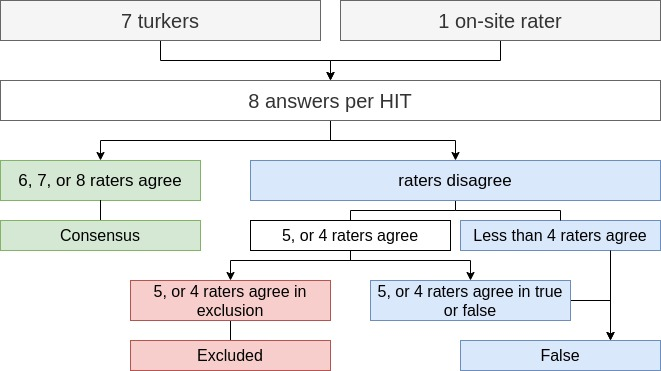
\includegraphics[width=0.8\linewidth]{images/chapter_6/figure_3.jpg}
\caption[Flowchart Illustrating How to Reach Majority Consensus]{Flowchart illustrating how to reach majority consensus, according to the answers provided by the workers plus our extra rater on site.} \label{fig3}
\end{figure}

To further assess the quality and challenges of curating the PGR dataset and validate the previous approach, a domain expert with a Bioinformatics background and experience in using and curating corpora also curated the relations in Task 2. 

\paragraph{Deep Learning Systems}

To further access the quality of the crowdsourced curated dataset, we applied it to two distinct deep learning systems that target the biomedical domain: BiOnt \citep{sousa2020biont} and BioBERT \citep{lee2020biobert}. For comparison, we tested both the original PGR dataset and the crowdsourced Amazon dataset, as well as combinations between the two (detailed in Table \ref{tab5}).

The BiOnt system is a deep learning system based on the BO-LSTM system \citep{lamurias2019bo} that is used to extract and classify relations via long short-term memory networks and biomedical ontologies. This system detects and classifies ten types of biomedical relations, such as human phenotype-gene relations. It takes advantage of domain-specific ontologies, like the Human Phenotype Ontology (HPO) \citep{kohler2017human} and the Gene Ontology (GO) \citep{ashburner2000gene}. The BiOnt system represents each entity as the sequence of its ancestors in their respective ontology.

The BioBERT system is a pre-trained biomedical language representation model for biomedical text mining based on the BERT \citep{devlin2019bert} architecture. This system can perform diverse biomedical text mining tasks, namely NER, RE, and Question Answering (QA), when trained on large-scale biomedical corpora. The novelty of the architecture is that their authors designed these systems (BioBERT and BERT) to pre-train deep bidirectional representations by joint conditioning on both the left and right context in all layers. This feature allows easy adaptation to several tasks without loss in performance.

\section{Results and Discussion}

\subsection{Ratings Statistics}

To assess the performance of the workers, we conducted some statistical analyses, including the time spent on average rating each sentence. Figure \ref{fig4} and \ref{fig5} reflect the average time spent by the workers with each sentence, with a cutoff of 50 seconds (using box plot and standard deviation analysis). We decided to set the cutoff for work time to 50 seconds because we considered that was enough time for a worker to make an assessment, and anything longer than that was probably the worker having a mid-task break (the longest time for a HIT completion was 40322 seconds, about 11 hours). 

\begin{figure}[H]
\centering
\begin{minipage}{0.48\textwidth}
\centering
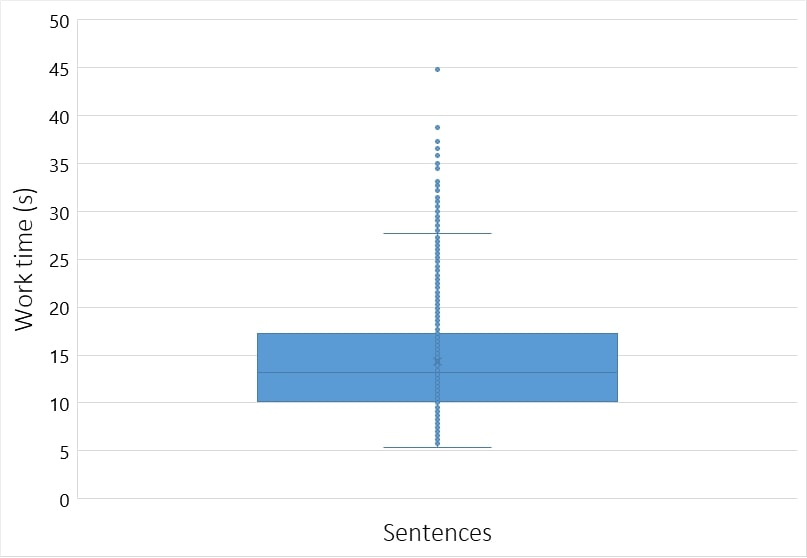
\includegraphics[width=0.97\linewidth]{images/chapter_6/figure_4.jpg}
\caption[Box Plot Expressing the Average Worker Work Time Distribution]{Box plot expressing the average worker work time distribution (in seconds) per sentence (with a cutoff of 50 seconds).}\label{fig4}
\end{minipage}
\hfill
\begin{minipage}{0.48\textwidth}
\centering
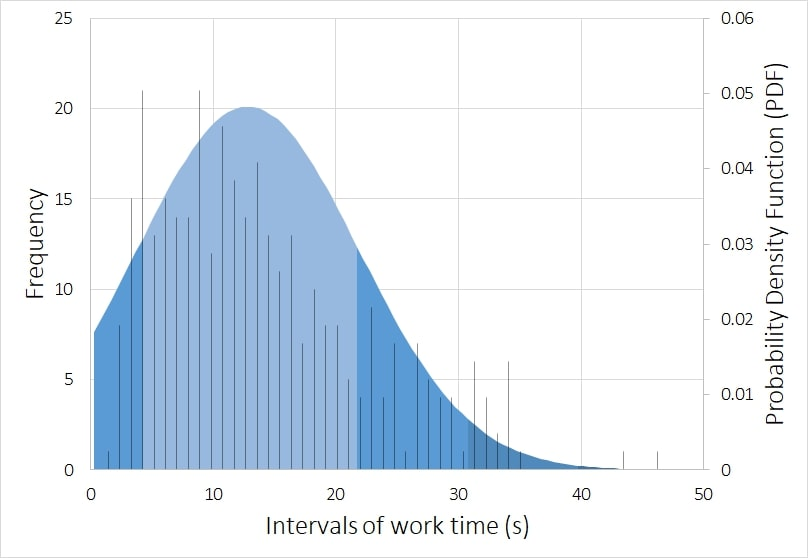
\includegraphics[width=0.97\linewidth]{images/chapter_6/figure_5.jpg}
\caption[Standard Deviation Expressing the Average Worker Work Time Distribution]{Standard deviation expressing the average worker work time distribution (in seconds), and the histogram of the occurrence events (with a cutoff of 50 seconds).}\label{fig5}
\end{minipage}
\end{figure}

Our domain expert did a similar time self-evaluation, which resulted in an average of about 20 seconds per sentence (for Task 2). The domain expert consulted some abstracts to clarify whether an abbreviation refers to a gene or other type of entity for a specific sentence. Through Figures \ref{fig4} and \ref{fig5}, it is possible to assess that workers took an average of 13 seconds per HIT (sentence). By comparing this time to the average time taken by our domain expert (20 seconds), it is possible to question the level of attention with which our workers performed their ratings, questioning the trust that we can deposit in MTurk crowdsourcing. However, taking into consideration that our domain expert took some time checking some abstracts to which workers did not have access, it can justify the differences in average time.

To further characterize the workers that performed our tasks, we checked their WorkerId tab in the results file provided by MTurk. There, we realized that six sentences were rated but did not have an associated WorkerId and that both tasks (7983 relations, 22255 HITs) were performed by only 64 different workers, making, on average, 348 HITs per worker. Therefore, if we had a malicious worker that classified their respective HITs randomly, it would damage the whole dataset. The MTurk platform should guarantee a more diverse group of workers working on the same task since that is what employees expect, even to avoid some biased ratings or a more strict selection process.

\subsection{Inter-rater Agreement}

Table \ref{tab3} presents the inter-rater agreement score, using both Fleiss’ kappa \citep{mchugh2012interrater} and Krippendorff’s alpha \citep{krippendorff2011computing} metrics, for the dataset corresponding to Task 2, considering only the Amazon workers, the Amazon workers plus the extra rater (on-site), and the extra rater (on-site) plus the domain expert.

\begin{table}[h]
\centering
\caption[Inter-rater Agreement Scores]{The inter-rater agreement score, using both Fleiss’ kappa and  Krippendorff’s alpha metrics, considering only the Amazon workers, the Amazon workers plus the extra rater (on-site), and the extra rater (on-site) plus the domain expert (Task 2). AW stands for Amazon Workers}\label{tab3}
\begin{tabular}{lccc}
\hline
\multirow{2}{*}{Inter-rater agreement metric} & \multicolumn{3}{c}{Inter-rater agreement} \\
\cline{2-4}
& AW & AW + extra rater (on-site) & Extra rater (on-site) + expert \\
\hline
Fleiss' kappa & 0.2028 & 0.2050 & 0.6549 \\
Krippendorff’s alpha & 0.2029 & 0.2051 & 0.6550 \\
\hline
\end{tabular}
\end{table}

Given the small number of workers working on Task 2 (33) and the high number of sentences to rate (2389), it is challenging to find an inter-rater agreement metric that can return an accurate agreement value between the workers. Fleiss’ kappa metric assumes that the raters are deliberately chosen and fixed, while Krippendorff’s alpha metric is indicated when we have multiple raters and multiple possible ratings. Since none of the two cases is precisely right, we do not have a metric that fully expresses the results of our experiment with Task 2. We can say that probably the agreement between raters was only moderate (on a qualitative scale). Some of the reasons for moderate agreement could be difficulties in understanding the task, complex biomedical sentences that are beyond the scope of the average worker, or random answers provided by malicious workers. 

It was particularly interesting to have an extra rater (on-site) that could express doubts while performing the task. Some of these doubts could be the ones that the workers had, while others we considered to be beyond their expertise. For our on-site rater, one of the most prominent problems was if the gene entities tagged were, in fact, gene entities or their proteins products that frequently share the same names. One could argue that a relation between a gene product and a human phenotype implies a relation between a gene and a human phenotype. Nonetheless, the extra rater considered that these relations hold even if the mention was of a protein and not the gene if this distinction was not clear by the sentence (only when reading the abstract or full-text article) or if the gene name was not capitalized. This particular problem was not one that a person not familiar with Biochemistry related domains would have. However, assessing if an abbreviation that is used both as a gene name and in other biomedical topics (e.g., disease abbreviation) is a gene is a transversal problem for both the workers and our extra rater on-site. 

The difficulties that our extra-rater experienced are evident in the inter-rater agreement between this rater and our domain expert. One example sentence where they disagreed was:

\textit{While examining pedigrees of JEB patients with \textbf{LAMA3} mutations, we observed that heterozygous carriers of functional null mutations displayed subtle enamel pitting in the absence of \textbf{skin fragility} or other JEB symptoms.} (PMID:27827380)

where the domain expert considered a true relation and the extra-rater a false relation, this happens because the relation is one of negation (absence) which often confuses non-experts with being false. However, an implication of relation of any sort is a true relation which can then be classified as positive or negative. This confusion is also noticeable by the diversity in the workers' answers for this sentence (four classified as true, two as false, and one as an error).
 
\subsection{Corpus Statistics}


Table \ref{tab4} presents the final numbers both in total count and percentage for each task. For Task 2, we considered the majority consensus described previously and the domain expert numbers separately.

\begin{table}[h]
\centering
\caption[Final Relations Counts]{The original and final numbers both in total count and percentage, for Tasks 1 and 2, of true, false, excluded and total relations, considering the majority consensus and the domain expert numbers separately. AW stands for Amazon Workers}\label{tab4}
\newcolumntype{A}{ >{\centering\arraybackslash} m{2cm} }
\begin{tabular}{lAcccc}
\hline
\multirow{2}{*}{Dataset} & & \multicolumn{4}{c}{Relations} \\
\cline{3-6}
\multicolumn{2}{c}{} & True & False & Excluded & Total\\
\hline
Task 1 (70\%) & Original & 1751 (31.41\%) & 3823 (68.59\%) & - & 5574 (100\%)\\
& AW & 4220 (75.71\%) & 283 (5.08\%) & 1071 (19.21\%) & 4503 (80.79\%)\\
\hline
Task 2 (30\%) & Original & 729 (30.51\%) & 1660 (69.49\%) & - & 2389 (100\%)\\
& AW + extra rater (on-site) (after reaching consensus) & 41179 (49.35\%) &613 (25.66\%) & 240 (10.05\%) & 1792 (75.01\%)\\
& Expert & 1281 (53.62\%) & 343 (14.36\%) & 765 (32.02\%) & 1624 (67.98\%)\\
\hline
\end{tabular}
\end{table}

From analyzing Table \ref{tab4}, what becomes immediately evident is the inversion between the number of true and false relations from the original datasets to the Amazon crowdsourced datasets. These final numbers demonstrate quite clearly that most relations described in the original PGR dataset as false were, in fact, true. This inversion can be due to how the PGR dataset was built, using a gold standard knowledge base of human phenotype-gene relations. This knowledge base, at the time of the dataset creation, was quite incomplete since, for instance, if a child's ontological term had a relation with a gene, its immediate parent would not necessarily share the same relation, which should be explicit. Thus, these parent concepts in PGR relations would always hold false. 

Also, understanding the difference between an annotation error and a false relation requires more expertise than the one that MTurk provides and that inexperienced raters have (even if in the field). Thus, to differentiate between false relations and an annotation error, we need expert knowledge, such as in the following annotation error example:

\textit{We show that the \textbf{miR}-106b-25 cluster upregulates NOTCH1 in multiple breast \textbf{cancer} cell lines, representing both estrogen receptor (ER+) and triple negative breast cancer (TNBC) through direct repression of the E3 ubiquitin ligase, NEDD4L.} (PMID:29662198)

where the workers had difficulties accessing that miR just by itself is not a gene entity but stands for microRNA genes (a large group of genes).

\subsection{Deep Learning Impact}

Table \ref{tab5} presents the performance of both the original PGR dataset and the crowdsourced Amazon dataset, and combinations between the two, on the BiOnt \citep{sousa2020biont} and BioBERT (version 1.1) \citep{lee2020biobert} systems, in terms of precision, recall, F-measure, and accuracy. To assess the performance of the dataset (before and after crowdsourcing) when applied to deep learning systems, we used the suggested parameters by the authors of each system. The only exception to the default parameters, since we had a class imbalance, was to add a class weight of 5 to the label false to both systems (the full multiplier to balance was approximately 14.9 for the Task 1 dataset). The full multiplier is a result of dividing the percentage of true relations by the percentage of false relations for the training dataset. For the class weight, we chose a number between 1 and the full multiplier, which is usually the standard practice \citep{chen2018efficient}, to maintain a more accurate representation of the natural unbalance between labels when applying the models to real-world data. Using this class weight translates to treating every training instance with the label false as five instances of the label true, meaning that in the loss function, we assign a higher value to these instances. Hence, the loss becomes a weighted average, where the weight of each sample is specified by the class weight and its corresponding class, providing a weight or bias for each output class. To achieve this, we had to alter the loss function of the BioBERT system to allow class weights.

\begin{table}[h]
\centering
\caption[Performance Metrics of BiOnt and BioBERT with the PGR Dataset]{Precision, recall, F-measure, and accuracy of the application of the PGR dataset (original, new, and combinations between the two) to the BiOnt and BioBERT systems. The highest scores for each metric are presented in bold}\label{tab5}
\newcolumntype{B}{ >{\raggedright} m{5cm} }
\begin{tabular}{lBcccc}
\hline
Method & & Precision & Recall & F-measure & Accuracy \\
\hline
BiOnt & PGR & 0.8140 & 0.3070 & 0.4459 & 0.4821\\
& Amazon (train) + PGR (test) & 0.7000 & 0.9825 & 0.8175 & 0.7024\\
& Amazon (train) + Amazon workers consensus (test) & 0.6810 & 0.9670 & 0.7992 & 0.6726\\
& Amazon (train) + Expert (test) & \textbf{0.8142} & 0.9721 & \textbf{0.8861} & \textbf{0.7989}\\
& Amazon workers consensus (train) + PGR (test) & 0.6880 & 0.8509 & 0.7608 & 0.6369\\
& Expert (train) + PGR (test) & 0.6894 & \textbf{0.9737} & 0.8072 & 0.6845\\
\hline
BioBERT & PGR & \textbf{0.8542} & 0.3445 & 0.4910 & 0.5143\\
& Amazon (train) + PGR (test) & 0.6744 & 0.9856 & 0.8000 & 0.6775\\
& Amazon (train) + Amazon workers consensus (test) & 0.6700 & 0.9763 & 0.7946 & 0.6680\\
& Amazon (train) + Expert (test) & 0.8103 & \textbf{0.9906} & \textbf{0.8915} & \textbf{0.8096}\\
& Amazon workers consensus (train) + PGR (test) & 0.7315 & 0.9160 & 0.8134 & 0.7143\\
& Expert (train) + PGR (test) & 0.7857 & 0.8319 & 0.8082 & 0.7314\\
\hline
\end{tabular}
\end{table}

The deep learning systems performance is quite similar, with BioBERT achieving slightly better results. In both systems, the performance of the new PGR dataset (through MTurk crowdsourcing) was superior to that of the original PGR dataset, with a slight decrease in precision but a considerable gain in the recall. We included the accuracy metric to consider the ability to recognize true negatives as well (due to the class imbalance). The best performance overall was the Amazon MTurk (Task 1) as the training corpus and the expert (Task 2) as the test corpus. This performance can be due to the amount of available training data in Task 1 and the more reliable test set from the domain expert. The PGR original test set underperformed probably due to its small size, which was not being representative of the data (260 relations).  Also, other experiences with using the majority consensus (Task 2) and the expert (Task 2) as training sets showed that these smaller corpora also hold the ability to train a model. 

\section{Conclusion and Future Directions}

This work describes our proposal for a complete pipeline for RE crowdsourcing. The pipeline  generated an openly available new release of the PGR dataset, as well as a domain expert revision into 30\% of the original dataset. Additionally, we assessed MTurk workers' performance by comparing them to an extra rater on-site and to a domain expert.   Moreover, we applied the new dataset as training data in two state-of-the-art deep learning systems (BiOnt \citep{sousa2020biont} and BioBERT \citep{lee2020biobert}) to measure the usefulness of the annotations. This study showed that it is possible to use the wisdom of the crowd to at least improve existing silver standard datasets since, in our case, it was able to exclude previous annotation errors (16.46\%) and modify wrongly labelled relations. This improvement had a significant impact on model training since we had a 0.3494 average increase in F-measure, taking into account all the experiences when comparing it with the original PGR dataset. 

Regarding future work, it will be interesting to improve on the existing pipeline by providing different guidelines and assessing if that would make a difference in performance. Also, we can differentiate between what constitutes a false and a negative relation. To solve the lack of domain expertise of MTurk workers, we could create a specialized crowdsourcing platform for the RE biomedical field, similar to the one developed by the company Unbabel that focuses on translation \citep{gracca2018unbabel}, as well as other biomedical crowdsourcing projects \citep{tsueng2020applying,kleffner2017foldit}. Finally, we could apply the same methods to datasets from other biomedical domains and assess the differences in performance. 

\clearpage
\section{Supplementary Material}


\begin{figure}[h]
\centering
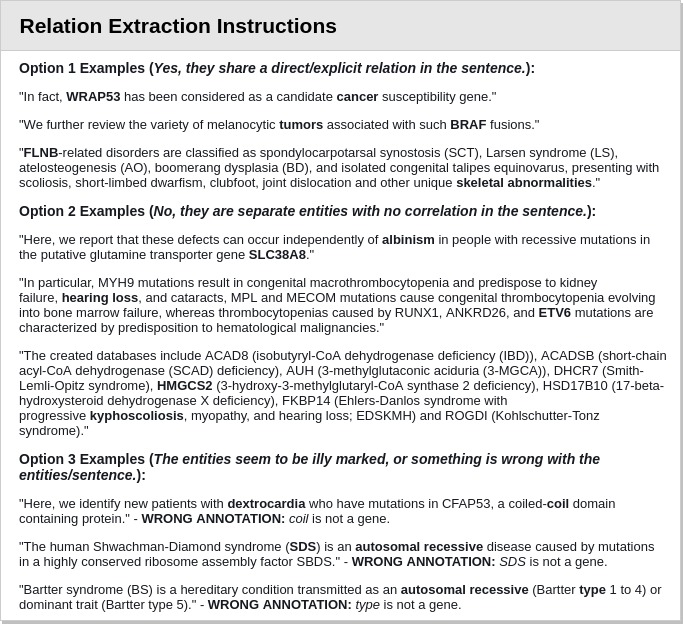
\includegraphics[width=0.8\linewidth]{images/chapter_6/supplementary_material_figure_1.jpg}
\caption[Amazon MTurk Guidelines]{The guidelines, in the form of examples of answers to different annotations, that were presented to the workers.} \label{sfig1}
\end{figure}

